% arara: pdflatex
% arara: convert: {density: 160, otheroptions: -dispose previous -delay 10 -loop 1, format: gif}
% arara: showfile: {format: gif}
\documentclass{article}
\usepackage{geometry}
\geometry{papersize={128mm,96mm}}
\usepackage{tikzducks}
\pagestyle{empty}
\newcommand{\frenchduck}{\begin{scope}[scale=.7]
	\clip (0,0) -- ++(2.2,0) -- ++(0,2.6) -- ++(-2.2,0) -- cycle;	
	\duck[body=yellow!60!red!30!white,tshirt=white!90!
	yellow,stripes={\stripes[color=blue!70!black,rotate
		=-87,width=0.07,distance=0.12]},beret=blue!30!black
	,baguette=brown]
	\end{scope}}

\begin{document}
	\begin{figure}
	\centering
	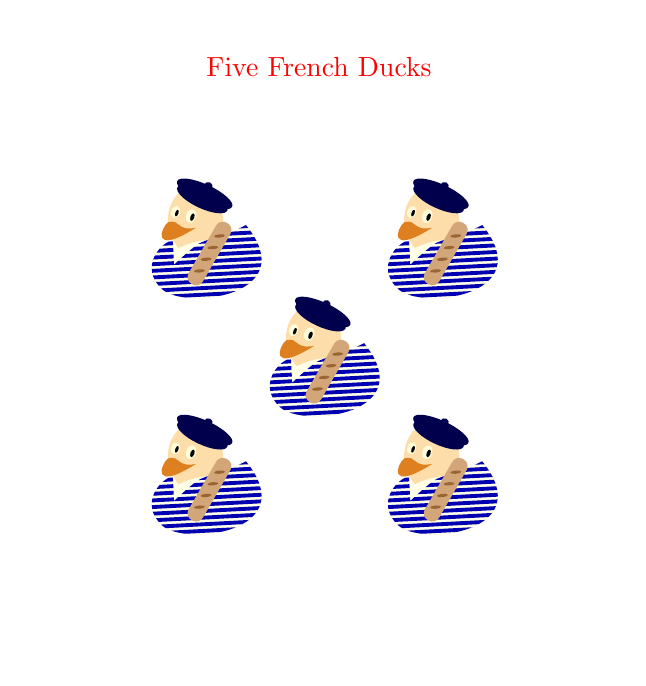
\begin{tikzpicture}
		\path (-3,-3) rectangle (4.5,5);
		\node[red] at (.7,4.5) {Five French Ducks};
		\frenchduck	
		\foreach \x in {-1.5,1.5} {%
			\foreach \y in {-1.5,1.5} {%
				\begin{scope}[shift={(\x, \y)}]
				\frenchduck
				\end{scope}
			}
		}
	\end{tikzpicture}	
	\end{figure}
	\begin{figure}
		\centering
		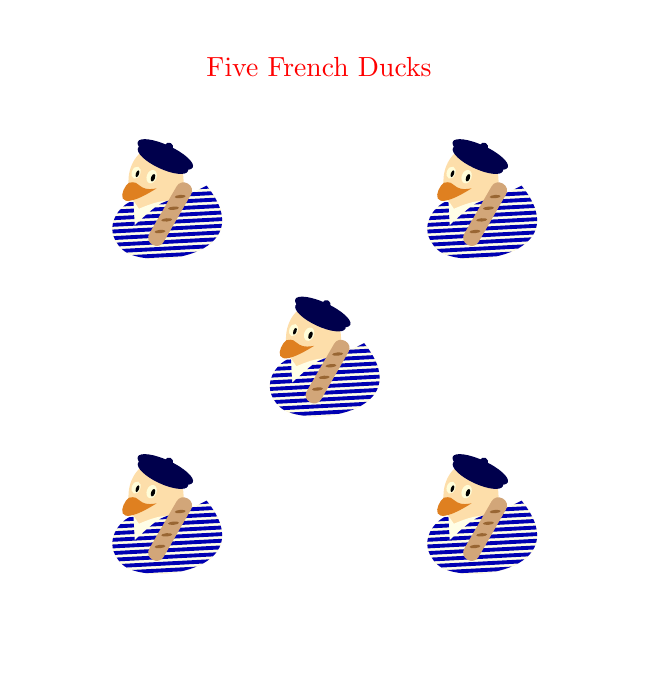
\begin{tikzpicture}
		\path (-3,-3) rectangle (4.5,5);
		\node[red] at (.7,4.5) {Five French Ducks};
		\frenchduck	
		\foreach \x in {-2,2} {%
			\foreach \y in {-2,2} {%
				\begin{scope}[shift={(\x, \y)}]
				\frenchduck
				\end{scope}
			}
		}
		\end{tikzpicture}	
	\end{figure}
	\begin{figure}
		\centering
		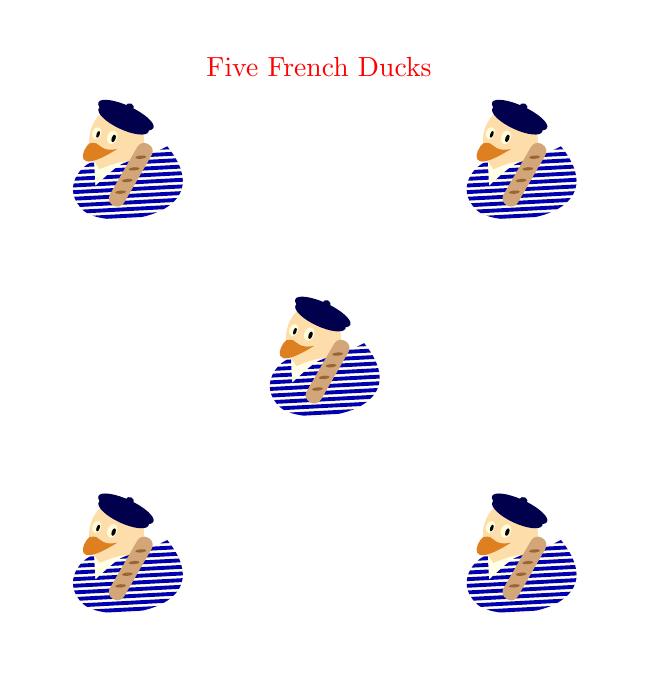
\begin{tikzpicture}
		\path (-3,-3) rectangle (4.5,5);
		\node[red] at (.7,4.5) {Five French Ducks};
		\frenchduck	
		\foreach \x in {-2.5,2.5} {%
			\foreach \y in {-2.5,2.5} {%
				\begin{scope}[shift={(\x, \y)}]
				\frenchduck
				\end{scope}
			}
		}
		\end{tikzpicture}	
	\end{figure}
\end{document} 